%% LyX 2.0.6 created this file.  For more info, see http://www.lyx.org/.
%% Do not edit unless you really know what you are doing.
\documentclass[letterpaper,twoside,italian]{article}
\usepackage{times}
\usepackage[scaled=0.9]{helvet}
\renewcommand{\ttdefault}{mathptmx}
\usepackage[T1]{fontenc}
\usepackage[utf8x]{inputenc}
\setcounter{secnumdepth}{-2}
\usepackage{graphicx}

\makeatletter

%%%%%%%%%%%%%%%%%%%%%%%%%%%%%% LyX specific LaTeX commands.
\special{papersize=\the\paperwidth,\the\paperheight}


%%%%%%%%%%%%%%%%%%%%%%%%%%%%%% User specified LaTeX commands.

\usepackage[italian]{babel}
\usepackage{url}
\title{Manuale utente del plugin Web Librarian}
%% There is no 'translator' parameter for the article class.
%%\translator{Lorenzo Novaro}
%% Putting the translation credit in the author field.
%% (Alternatively, it could be defined with the \thanks variable, in which 
%% case it will appear as a footnote to the title.)
\author{Robert Heller (Italian translation by Lorenzo Novaro)}
%% lifted from generic/babel/italian.ldf
\renewcommand{\contentsname}{Indice}
\def\today{\number\day~\ifcase\month\or
     gennaio\or febbraio\or marzo\or aprile\or maggio\or giugno\or
     luglio\or agosto\or settembre\or ottobre\or novembre\or
     dicembre\fi\space \number\year}%
\date{\today}


\makeatother

\usepackage{babel}
\begin{document}
\maketitle

\tableofcontents{}


\section{Introduzione}

Questo plugin è nato come sistema portatile e multipiattaforma per
l'utilizzo da parte della Wendell Free Library durante la migrazione
dal precedente sistema basato su schede cartacee a quello che prima
o poi verrà fornito dal sistema bibliotecario regionale. Si è poi
trasformato nell'erede web-based del programma Home Librarian 3 della
Deepwoods Software.

Il plugin offre una gestione bibliotecaria web-based semplice e immediata,
completa di catalogazione e sistema di prestito. Per ricercare e visualizzare
elementi della collezione, potete usare gli shortcode disponibili.
Ci sono anche diverse pagine di amministrazione dove potete gestire
la collezione, gli iscritti della biblioteca e il banco prestiti.


\section{Installazione e configurazione iniziale}

Il plugin può essere installato direttamente caricando il file zip
o usando l'installazione automatica dall'interfaccia di WordPress.

Ci sono delle opzioni che possono essere impostate, ma non sono necessarie
per il funzionamento di base.


\subsection{Configurazione opzioni}

Sono presenti tre opzioni, tutte correlate all'suo dei web service
di Amazon. Un account Amazon vi può tornare utile se intendete ricercare
informazioni sugli elementi della tua collezione. Per fare ciò vi
serviranno una chiave pubblica ed una privata per i web service di
Amazon. Vi servirà anche un Amazon Associate Tag. Una volta ottenute
tali chiavi, dovrete impostare correttamente le configurazioni: 
\begin{enumerate}
\item \textbf{Chiave pubblica AWS} È la chiave pubblica che usi per accedere
ai web service di Amazon. 
\item \textbf{Chiave privata AWS} È la tua chiave privata per i web service
di Amazon. 
\item \textbf{Regione AWS} È la regione da usare per i web service di Amazon. 
\item \textbf{Amazon Associate Tag} È la Amazon Associate Tag da usare. 
\end{enumerate}
Per utilizzare le funzioni di ricerca di Amazon è necessario impostare
tutte e \textbf{quattro}.


\subsection{Impostazione dei ruoli utente}

Web Librarian aggiunge tre privilegi:
\begin{enumerate}
\item \textbf{manage\_patrons} Permette di aggiungere, modificare ed eliminare
gli iscritti. 
\item \textbf{manage\_collection} Permette aggiungere, modificare ed eliminare
gli elementi della collezione. 
\item \textbf{manage\_circulation} Permette la gestione dei prestiti e la
prenotazione di elementi. 
\end{enumerate}
E tre ruoli di utenza: 
\begin{enumerate}
\item \textbf{Bibliotecario} Il ruolo di bibliotecario comprende tutti i
privilegi menzionati, più il privilegio \textbf{edit\_users}%
\footnote{Necessario per poter associare gli ID iscritto agli utenti del sito.%
}. Di solito questo ruolo viene assegnato al direttore della biblioteca. 
\item \textbf{Assistente} L'assistente riceve i privilegi \textbf{manage\_collection}
e \textbf{manage\_circulation} e così, oltre a poter gestire il banco
prestiti, può aggiungere, modificare ed eliminare gli elementi della
collezione. 
\item \textbf{Volontario} Il solo privilegio del volontario è \textbf{manage\_circulation},
che permette ad un volontario di gestire il banco prestiti. 
\end{enumerate}
Normalmente nelle piccole biblioteche solo il direttore o un bibliotecario
anziano hanno l'autorità di aggiungere, eliminare e modificare le
iscrizioni, visto che ciò regola anche l'accesso al prestito. Il ruolo
dell'assistente corrisponde ad una persona autorizzata a svolgere
mansioni di backoffice come gestire il banco prestiti e la collezione
ed è tipicamente impiegato in biblioteche più grandi. I volontari
sono persone che si possono occupare del banco prestiti e segnare
quali elementi della collezione sono fuori e quali rientrano. Nel
caso di biblioteche molto piccole tutti questi ruoli potrebbero essere
ricoperti da una sola persona (il bibliotecario). Nota bene: tale
utente non corrisponde all'amministratore del sito WordPress.


\subsection{Shortcode per accedere alla collezione dalle pagine del sito}

Dovrete creare delle pagine e inserirvi dentro uno o più degli shortcode
disponibili, se volete rendere visibile e ricercabile la collezione
dal vostro sito o blog. Attualmente sono disponibili tre shortcode: 
\begin{enumerate}
\item \textbf{weblib\_searchform} Questo codice genera un modulo per effettuare
ricerche nella collezione. Accetta i seguenti parametri: 

\begin{description}
\item [{name}] Il titolo del modulo. Quello predefinito è `searchform'. 
\item [{actionurl}] Indirizzo di destinazione per il modulo. il valore
predefinito è `' (Ciò significa che i risultati verranno mostrati
sulla pagina stessa). 
\item [{method}] Il metodo del modulo. Il valore predefinito è `GET'. 
\end{description}

Si possono effettuare ricerche per titolo, autore, argomento, parole
chiave e codice ISBN. I risultati possono venire ordinati per codice
interno, titolo o autore, in ordine discendente o ascendente.


I parametri seguenti saranno passati alla pagina di destinazione: 
\begin{description}
\item [{searchby}] Il campo per cui effettuare la ricerca. I valori validi
sono: title (titolo), author (autore), subject (argomento), keyword
(parola chiave), o isbn. 
\item [{searchbox}] Testo della ricerca. 
\item [{webliborderby}] Il campo di ordinamento dei risultati. I valori
validi sono: barcode (codice a barre), title (titolo), o author (autore). 
\item [{webliborder}] Il tipo di ordinamento: ASC o DESC. 
\end{description}
\item \textbf{weblib\_itemlist} Questo shortcode genera una lista di risultati
processando i risultati generati da \textbf{weblib\_searchform}. Accetta
i seguenti parametri: 

\begin{description}
\item [{name}] Il nome da dare al div contenente la lista degli elementi.
Il valore predefinito è `itemlist'. 
\item [{perpage}] Il numero di elementi da mostrare su ogni pagina. Il
valore predefinito è 10. 
\item [{moreinfourl}] L'indirizzo della pagina contenente informazioni
dettagliate per un elemento selezionato. Il valore predefinito è `'. 
\item [{inlinemoreinfo}] Se impostato come `true' (vero), questo shortcode
visualizzerà le informazioni dettagliate di un elemento selezionato.
Il valore predefinito è `false'. 
\item [{holdbutton}] Se impostato come `true' e se l'utente è collegato
ad un id iscritto, questo shortcode fa apparire un pulsante che permette
la prenotazione degli elementi trovati. Il valore predefinito è `false' 
\end{description}

Questo codice richiama \textbf{weblib\_itemdetail} per generare elenchi
di elementi trovati visualizzati in breve o (se \textbf{inlinemoreinfo}
è impostato come `true') per generare la visualizzazione dettagliata
dell'elemento selezionato (o del solo elemento trovato). 

\item \textbf{weblib\_itemdetail} Questo codice mostra un elemento in modo
più o meno dettagliato. Di solito viene inserito in una pagina a sè
stante (per esempio quella collegata a \textbf{moreinfourl} passata
a \textbf{weblib\_itemlist}). Accetta i seguenti parametri: 

\begin{description}
\item [{name}] Il nome del div contenitore. Il nome predefinito è `itemdetail{[}\%i{]}';
il \%i viene sostituito automaticamente con il codice a barre dell'elemento. 
\item [{barcode}] Il codice a barre dell'elemento da visualizzare. Il valore
predefinito è `'. 
\item [{getbarcode}] Se impostato come `true' (vero), questo shortcode
otterrà il codice a barre dai parametri CGI. Viene solitamente utilizzato
con il parametro \textbf{moreinfourl} dello shortcode \textbf{weblib\_itemlist}.
Il valore predefinito è true. 
\item [{holdbutton}] Se impostato come `true' e se l'utente è collegato
ad un id iscritto, verrà visualizzato un pulsante per la prenotazione
degli elementi. Il valore predefinito è false. 
\item [{detaillevel}] Livello di dettaglio della visualizzazione. Impostandolo
su `sintetico' (il valore predefinito) verranno visualizzati pochi
dettagli. Ciò è utile nel caso di un lungo elenco di elementi (viene
utilizzato dallo shortcode \textbf{weblib\_itemlist} per la visualizzazione
di risultati multipli). Impostandolo su `esteso' verranno visualizzati
molti più dettagli (è ciò che fa lo shortcode \textbf{weblib\_itemlist}
per la visualizzazione di un singolo risultato). 
\item [{moreinfourl}] URL della pagina dove sono visualizzate le informazioni
riguardanti l'elemento. Il valore predefinito è `'. 
\end{description}

Shortcode richiamato dallo shortcode \textbf{weblib\_itemlist}. Non
è da utilizzare direttamente, a meno che non si voglia mettere in
risalto un elemento selezionato, usando una pagina apposita. 

\end{enumerate}

\subsubsection{Semplice esempio}

\begin{figure}[htbp]
\begin{centering}
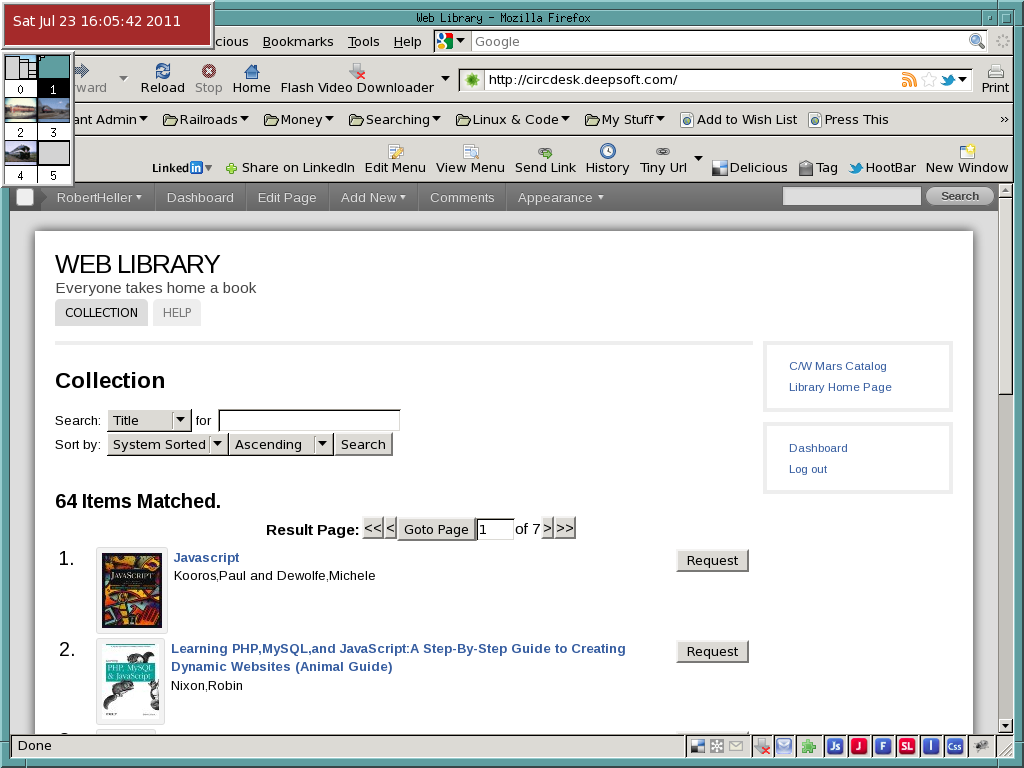
\includegraphics[width=4in]{frontside} \caption{Lista di risultati in visualizzazione sintetica}

\par\end{centering}

\centering{}\label{fig:frontside} 
\end{figure}


\begin{figure}[htbp]
\begin{centering}
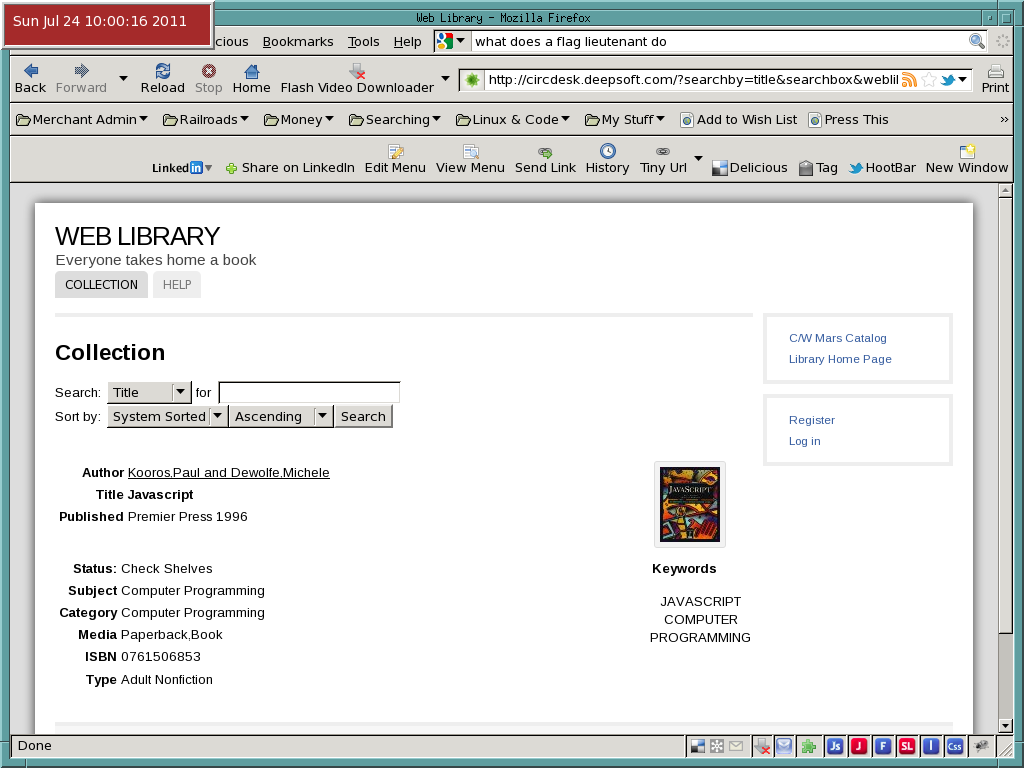
\includegraphics[width=4in]{frontone} \caption{Singolo elemento in visualizzazione estesa}

\par\end{centering}

\centering{}\label{fig:frontone} 
\end{figure}


Una pagina che includa il contenuto seguente è sufficiente per avere
un'interfaccia di ricerca nella collezione con visualizzazione dei
risultati. The results of this page are shown in Figures~\ref{fig:frontside}
and \ref{fig:frontone}.

\begin{verbatim} {[}weblibsearchform{]} {[}weblibitemlist holdbutton=1
inlinemoreinfo=1{]} \end{verbatim}


\section{Profile / User Management}

This plugin adds several pages to the user management / profile dashboard
pages, upto 3 for non-priviledged users and upto 4 for users with
`edit\_user' priviledge. These pages are: 
\begin{enumerate}
\item \textbf{Edit Patron Info} This page allows WordPress users to associate
a library patron id with their WordPress username and to edit their
patron name and contact information. 
\item \textbf{Holds} This page allows WordPress users who have an associated
library patron id to view their current list of holds (requests). 
\item \textbf{Checkouts} This page allows WordPress users who have an associated
library patron id to view their current list of checked out items. 
\item \textbf{Add Patron ID} This page allows priviledged users users (typically
librarians and adminstators) to associate patron ids with WordPress
users. 
\end{enumerate}

\subsection{Editing Your Patron Info}

\begin{figure}[htbp]
\begin{centering}
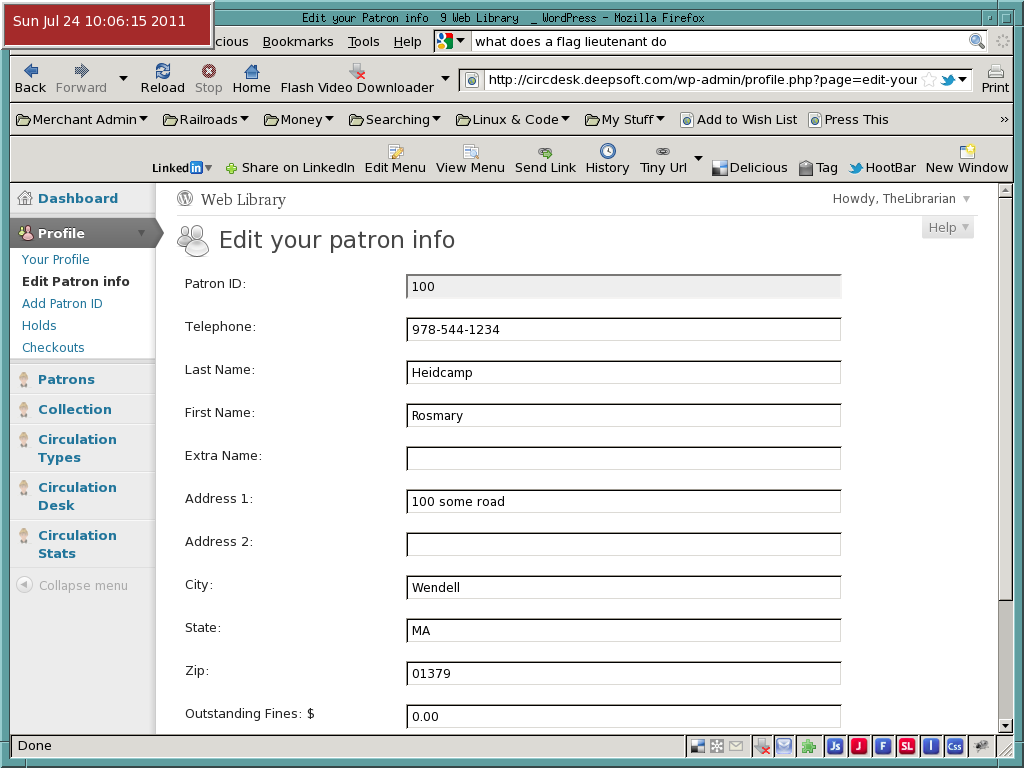
\includegraphics[width=4in]{EditPatronInfo} \caption{Editing Patron Info}

\par\end{centering}

\centering{}\label{fig:EditPatronInfo} 
\end{figure}


This page, shown in Figure~\ref{fig:EditPatronInfo} allows WordPress
users to first associate their WordPress username with a patron id
and then allows them to update their name and contact information.


\subsection{Items on Hold}

This page lists the items a patron has requested a hold on. The patron
can remove holds on selected items.


\subsection{Checked out items}

This page lists the items a patron has checked out. The due dates
are listed and the patron has the option of renewing items (up to
a limit of 2 renewals).


\subsection{Add Patron ID}

This page, which requires priviledge (\textbf{edit\_users}), allows
librarians and adminstators to associate (or disassociate) patron
ids with WordPress users.


\section{Patron Management}

\begin{figure}[htbp]
\begin{centering}
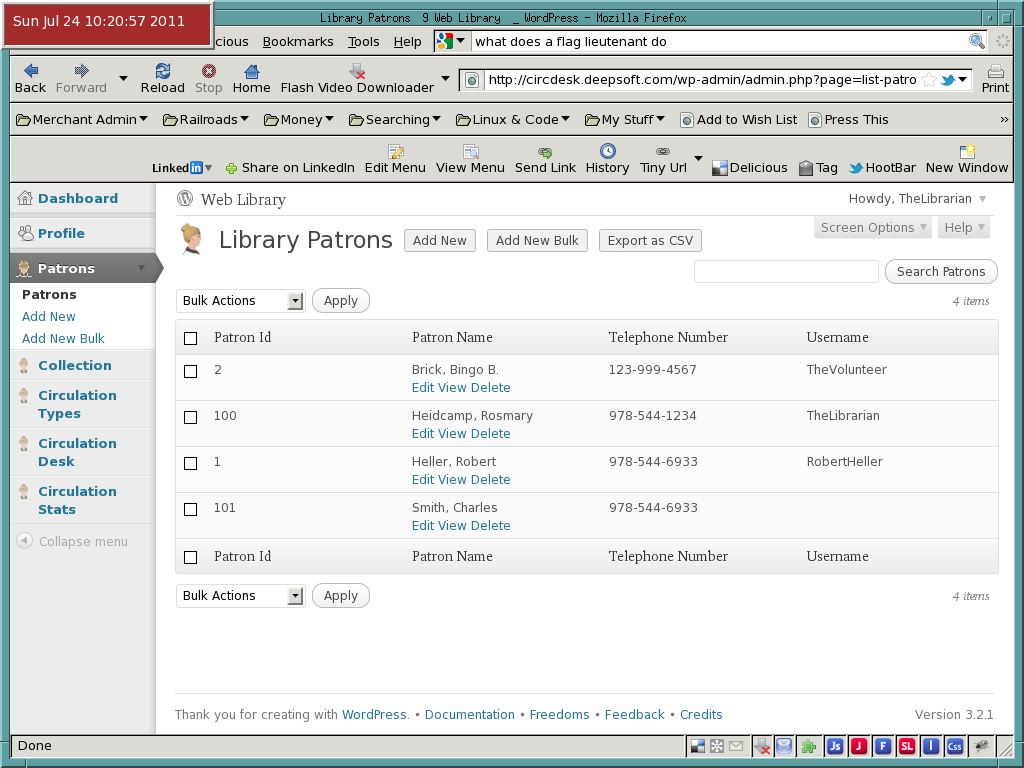
\includegraphics[width=4in]{PatronManagement} \caption{Patron List Page}

\par\end{centering}

\centering{}\label{fig:PatronList} 
\end{figure}


Patron management entails the adding, removing, and editing of patrons
and requires \textbf{manage\_patrons} priviledge. The main patron
management page, shown in Figure~\ref{fig:PatronList}, lists the
patrons in the database. Patrons can be added one at a time or in
bulk. Patrons can also be viewed or edited. Each patron has a unique
id number, which is used when patrons either request holds or checkout
items. Basic contact information is stored for each patron, as well
as any outstanding files. Each patron also has an expiration date.
Nothing special is done when the expiration date is passed. This is
a bookkeeping feature to allow librarians to cull inactive patrons.

The Patron database can be downloaded as a CSV file and Patrons can
be uploaded in bulk using a CSV file. The columns recognized are: 
\begin{description}
\item [{id}] The patron id. 
\item [{firstname}] The patron's first name. 
\item [{lastname}] The patron's last name. 
\item [{extraname}] The patron's extra name (usually middle name). 
\item [{address1}] The patron's first address line. 
\item [{address2}] The patron's second (optional) address line. 
\item [{city}] The patron's city. 
\item [{state}] The patron's state. 
\item [{zip}] The patron's zip code. 
\item [{telephone}] The patron's telephone number. 
\item [{outstandingfines}] The patron's outstanding fines. 
\item [{expiration}] The patron's expiration date. 
\end{description}
The minimum set of columns needed are \textbf{firstname}, \textbf{lastname},
\textbf{address1}, \textbf{city}, \textbf{state}, \textbf{zip}, and
\textbf{telephone}.


\section{Collection Database Management}

\begin{figure}[htbp]
\begin{centering}
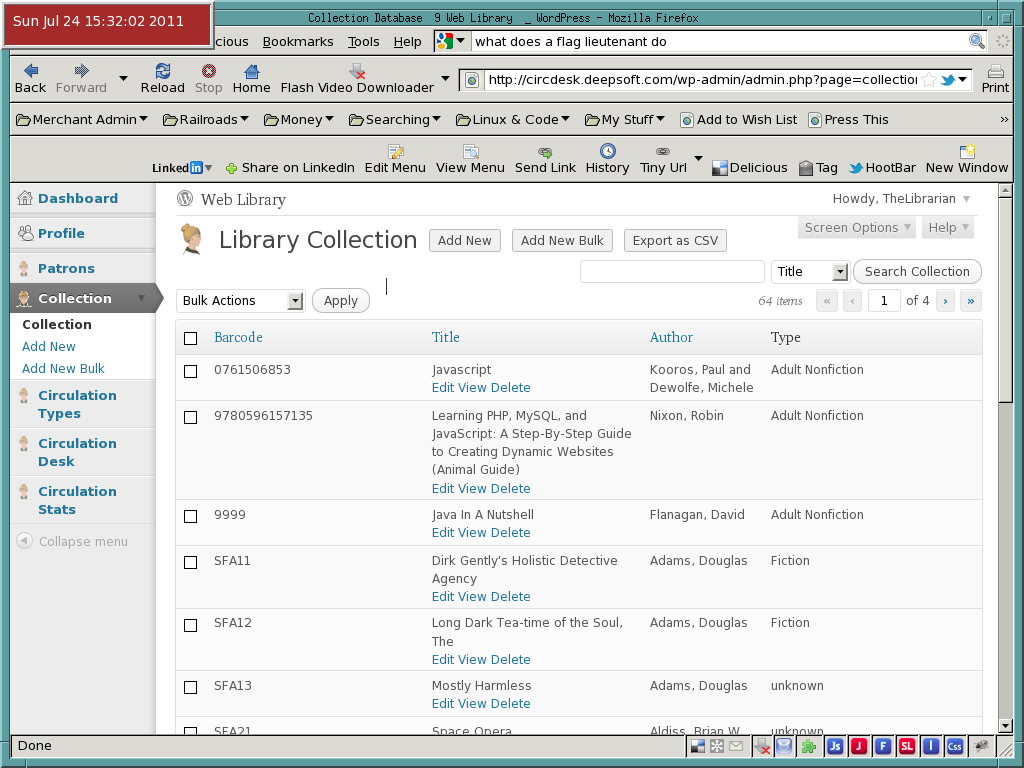
\includegraphics[width=4in]{ColectionListing} \caption{Collection Listing Page}

\par\end{centering}

\centering{}\label{fig:CollectionList} 
\end{figure}


Collection database management entails the adding, removing, and editing
of items in your collection and requires \textbf{manage\_collection}
priviledge. The main collection management page, shown in Figure~\ref{fig:CollectionList},
lists the items in your collection database. Items can be added one
at a time or in bulk and can be viewed or edited. Each item has a
unique ``barcode'', which is up to 16 characters long. Often this
is a digit string as returned by a barcode scanner, either from barcode
stickers printed or purchased for this purpose or from printed UPC
labels on the items themselves.

Items in the collection database can be searched by title, author,
subject, ISBN, or keyword. The rows can be worted by barcode, title,
or author. And the whole database can be exported as a CSV file.


\subsection{Adding and editing items in the collection database}

\begin{figure}[htbp]
\begin{centering}
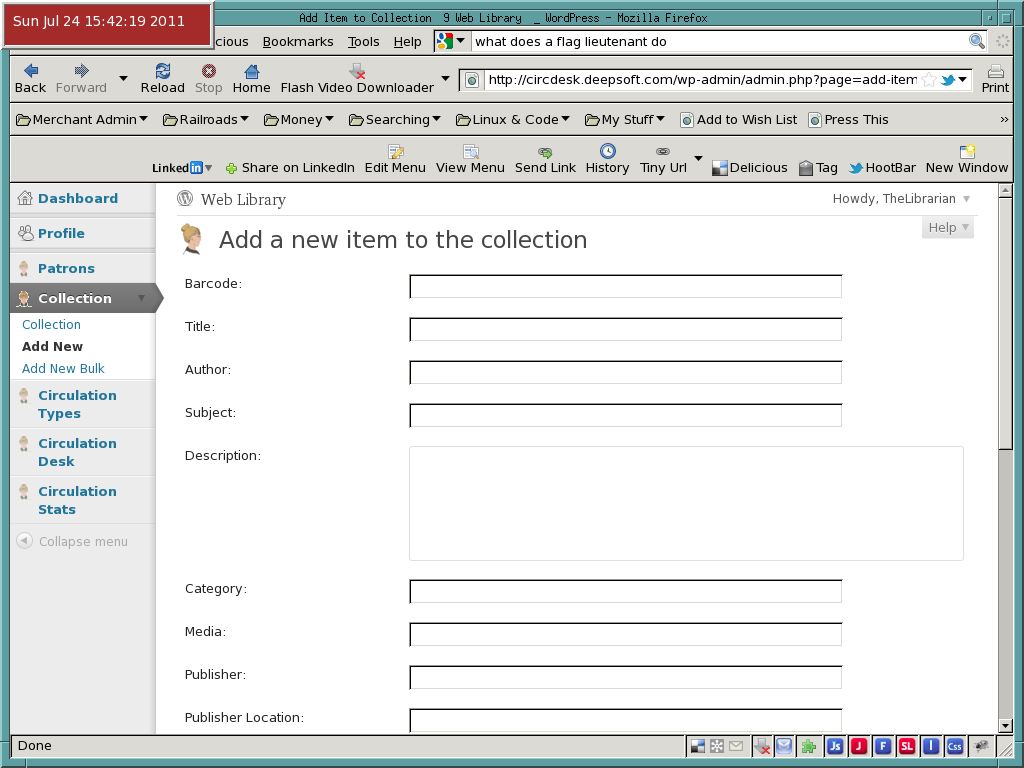
\includegraphics[width=4in]{AddItem} \caption{Adding an item to the collection}

\par\end{centering}

\centering{}\label{fig:AddItem} 
\end{figure}


\begin{figure}[htbp]
\begin{centering}
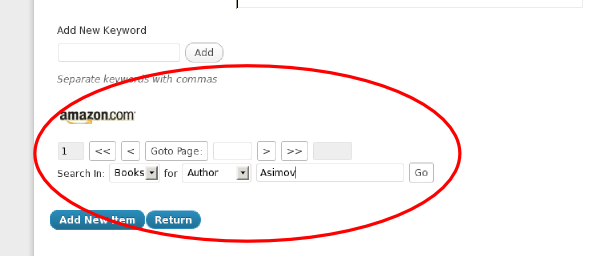
\includegraphics[width=4in]{AmazonSearch} \caption{Amazon Search Form}

\par\end{centering}

\centering{}\label{fig:AmazonSearch} 
\end{figure}


\begin{figure}[htbp]
\begin{centering}
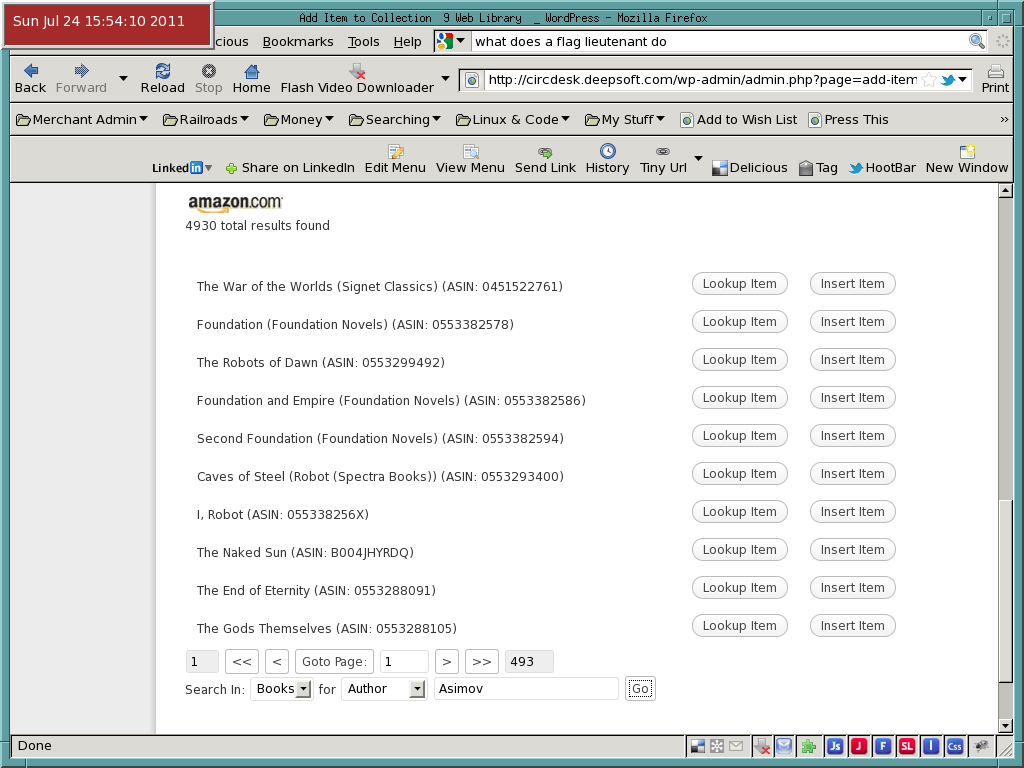
\includegraphics[width=4in]{AmazonSearchResults} \caption{Amazon Search Results}

\par\end{centering}

\centering{}\label{fig:AmazonSearchResults} 
\end{figure}


\begin{figure}[htbp]
\begin{centering}
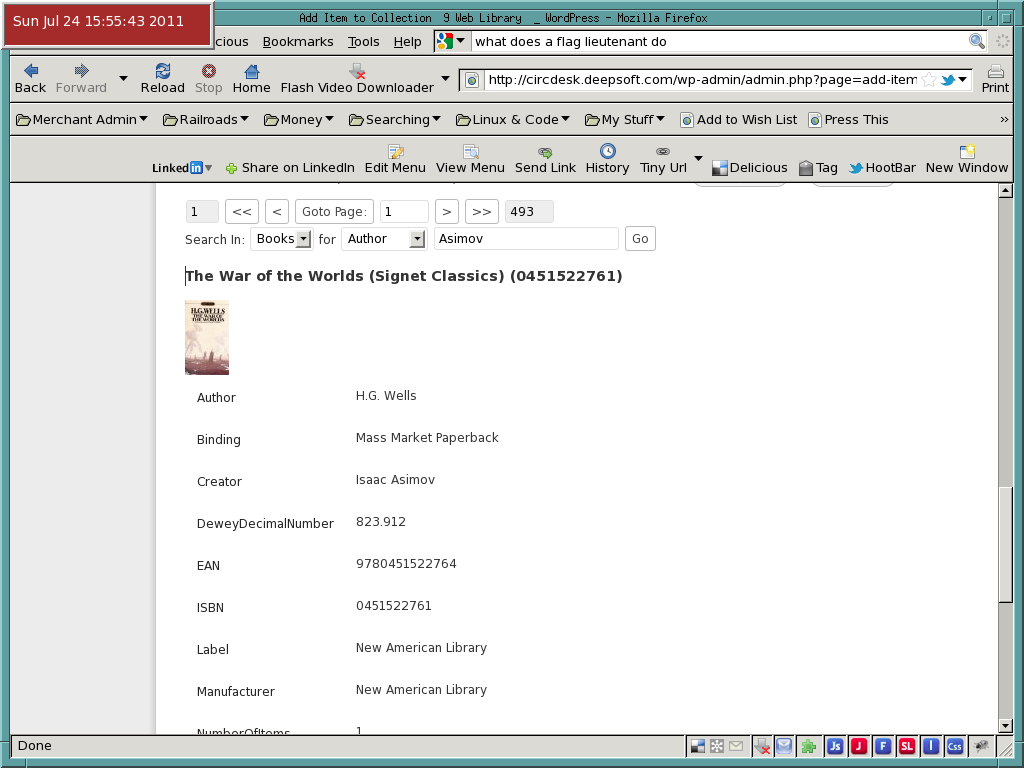
\includegraphics[width=4in]{AmazonLookupResults} \caption{Amazon Lookup Results}

\par\end{centering}

\centering{}\label{fig:AmazonLookupResults} 
\end{figure}


On the add item page, shown in Figure~\ref{fig:AddItem}, there are
fields for all of the database columns of an item, including Barcode,
Title, Author, Subject, Description, Category, Media, Publisher, Publisher
Location, Publish Date, Edition, ISBN, Type, Thumbnail URL, and Keywords.
Only the Title, Author, Subject, and Type are required. It is also
possible to make use of Amazon's extensive product database to find
values for or to directly fill in these fields. Under the Amazon logo
is a form for entering searches of Amazon's product database, shown
in Figure~\ref{fig:AmazonSearch}. Typical Amazon search results
are shown in Figure~\ref{fig:AmazonSearchResults} and item lookup
results are shown in Figure~\ref{fig:AmazonLookupResults}.


\subsection{Adding items in bulk to the collection database}

A CSV file can be uploaded to add items in bulk to the collection
database. The columns recognized are:
\begin{description}
\item [{barcode}] This is the item's barcode. 
\item [{title}] This is the item's title. It is required. 
\item [{author}] This is the item's author. It is required. 
\item [{subject}] This is the item's subject. It is required. 
\item [{description}] This is the item's description. 
\item [{category}] This is the item's category. 
\item [{media}] This is the item's media. 
\item [{publisher}] This is the item's publisher. 
\item [{publocation}] This is the item's publisher's location. 
\item [{pubdate}] This is the item's publish date. 
\item [{edition}] This is the item's edition. 
\item [{isbn}] This is the item's ISBN. 
\item [{type}] This is the item's type. It is required. 
\item [{thumburl}] This is the item's thumbnail URL. 
\item [{keywords}] This is the item's keywords (as a quoted, comma separated
list). 
\end{description}

\section{Circulation Type Management}

\begin{figure}[htbp]
\begin{centering}
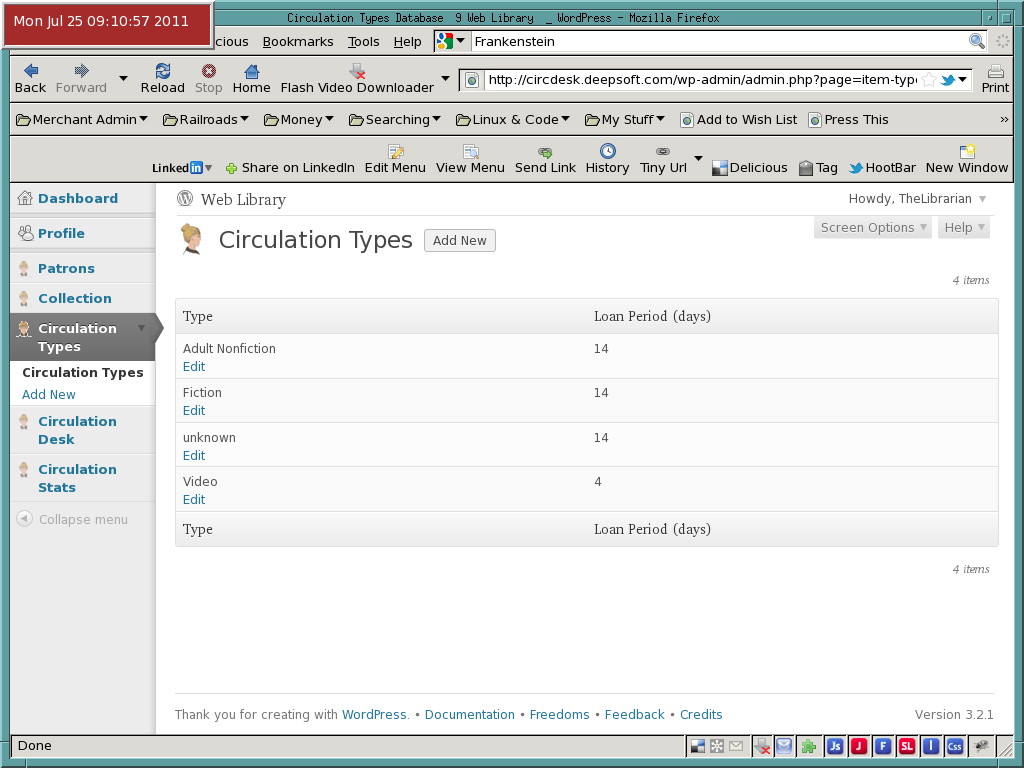
\includegraphics[width=4in]{CirculationTypesList} \caption{Circulation Types List page}

\par\end{centering}

\centering{}\label{fig:CirculationTypesList} 
\end{figure}


Items in the collection database have an associated \textit{Circulation
Type}, which defines a loan period and is also used for statistical
anaylsis. The circulation type management pages are used to manage
these \textit{Circulation Types}, where they can be listed (see Figure~\ref{fig:CirculationTypesList},
new ones added, and existing ones edited.


\section{Circulation Desk}

The \textit{Circulation Desk} page implements a virtual circulation
desk, where circulation tasks can be performs. These tasks consist
of checking out items, placing items on hold, checking in returns,
listing patron and item circulation records, listing items on hold,
and listing items checked out. There are six aspects of this page,
representing the six functional modes:
\begin{enumerate}
\item \textbf{Main Circulation} This is the general entry mode, and list
all items in the collection with their circulation status, described
in Section~\ref{sect:MainCirculation}. 
\item \textbf{Item Circulation Record} This mode list the circulation status
for a selected item in the collectection, described in Section~\ref{sect:ItemCirculationRecord}. 
\item \textbf{Patron Circulation Record} This mode lists the circulation
record for a selected patron. This is a listing of items this patron
has on hold or has checked out, described in Section~\ref{sect:PatronCirculationRecord}. 
\item \textbf{Circulation Hold List} This mode lists the items that currently
have holds on them, described in Section~\ref{sect:CirculationHoldList}. 
\item \textbf{Circulation Checkout List} This mode lists the items that
are currently checked out, described in Section~\ref{sect:CirculationCheckoutList}. 
\item \textbf{Circulation Checkin Page} This mode is used for checking in
returned items, described in Section~\ref{sect:CirculationCheckinPage}. 
\end{enumerate}

\subsection{Main Circulation}

\label{sect:MainCirculation}

\begin{figure}[htbp]
\begin{centering}
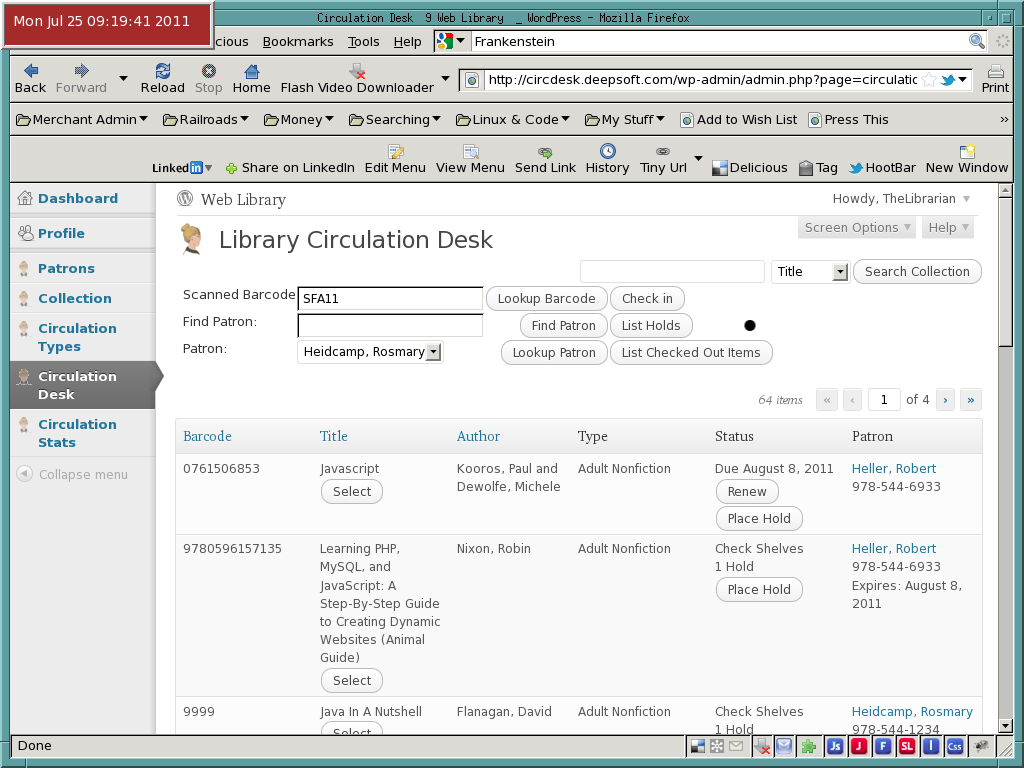
\includegraphics[width=4in]{MainCirculation} \caption{Main Circulation page}

\par\end{centering}

\centering{}\label{fig:MainCirculation} 
\end{figure}


The main circulation page is the initial aspect of the \textit{Circulation
Desk} page. It lists the the circulation records of all items%
\footnote{A page at a time.%
} in the collection. The same searching and ordering as is available
on the collection management page is available, as shown in Figure~\ref{fig:MainCirculation}.
From this aspect all of the other aspects can be selected, by use
of the various buttons at the top of the page: 
\begin{description}
\item [{Lookup Barcode}] This button looks up an item by barcode and displays
the selected items circulation record (see Section~\ref{sect:ItemCirculationRecord}). 
\item [{Lookup Patron}] This button looks up a selected patron and displays
the patron's circulation record (see Section~\ref{sect:PatronCirculationRecord}). 
\item [{Check in}] This button shifts to the returned items check in page,
as described in Section~\ref{sect:CirculationCheckinPage}. 
\item [{List Holds}] This button shifts to the circulation hold list aspect,
as described in Section~\ref{sect:CirculationHoldList}. 
\item [{List Checked Out Items}] This button shifts to the circulation
checked out list, as described in Section~\ref{sect:CirculationCheckoutList} 
\end{description}
\begin{figure}[htbp]
\begin{centering}
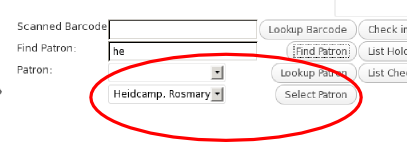
\includegraphics[width=4in]{FindPatron} \caption{Patron Search Results}

\par\end{centering}

\centering{}\label{fig:FindPatron} 
\end{figure}


There is an additional button, the \textbf{Find Patron} button. This
button does not change the page's aspect. Instead it does a search,
by name, of the patron database and displays a drop down list of matches,
from which a patron can be selected, as shown in Figure~\ref{fig:FindPatron}.

All of the item lists are same%
\footnote{Except for the \textit{Patron Circulation Record} listing, which ommits
the \textbf{Patron} column.%
}, listing the item barcode, the item title, the item author, the item
status, and the patron the item is checked out to or held by. If the
item is neither checked out nor held, this last column is blank. If
an item is both checked out and has a hold, the patron the item is
checked out to is listed. If the item has more than one hold, the
patron associated with the first (earliest) hold is listed. In the
title column is a \textbf{Select} button that can be used to directly
look up the item. If the item is checked out, there will be a \textbf{Renew}
button in its status column. There will always be a \textbf{Hold}
button in the status column, which will place a hold for the currently
selected patron.


\subsection{Item Circulation Record}

\label{sect:ItemCirculationRecord}

\begin{figure}[htbp]
\begin{centering}
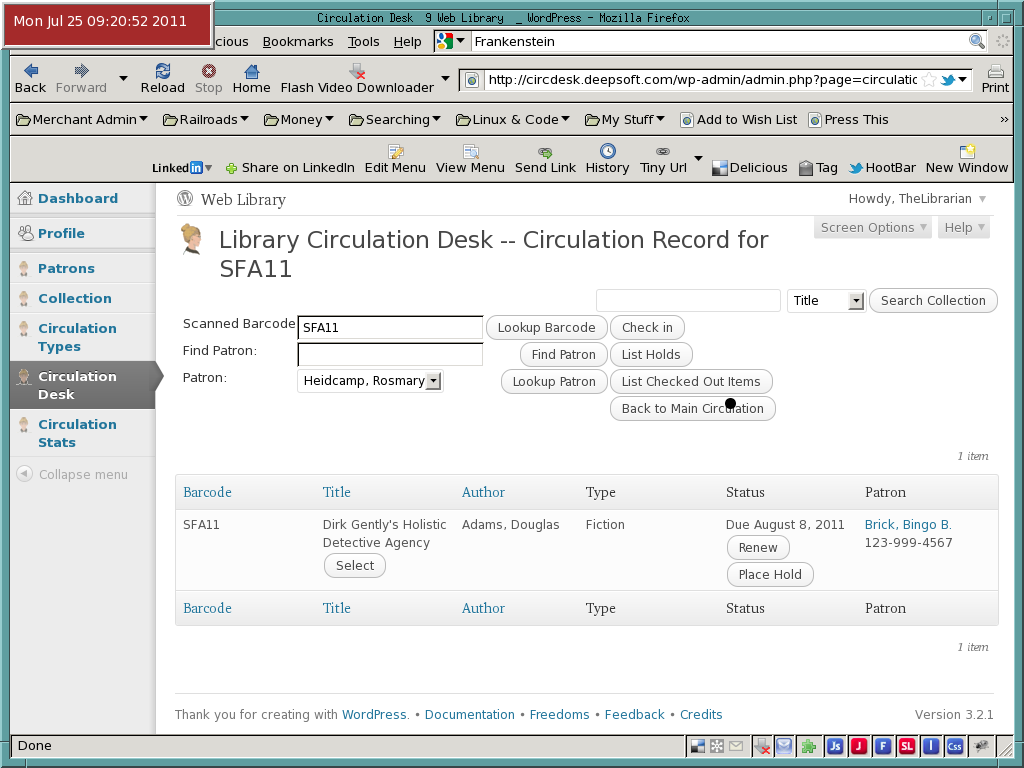
\includegraphics[width=4in]{ItemCirculationRecord} \caption{Circulation Record for a selected item (SFA11)}

\par\end{centering}

\centering{}\label{fig:ItemCirculationRecord} 
\end{figure}


This aspect of the \textit{Circulation Desk} page is shown when a
specific item has been looked up or selected. Only the selected item
is listed and an additional button is added to return to the main
aspect of the circulation desk page. A typical view of this page is
shown in Figure~\ref{fig:ItemCirculationRecord}.


\subsection{Patron Circulation Record}

\label{sect:PatronCirculationRecord}

\begin{figure}[htbp]
\begin{centering}
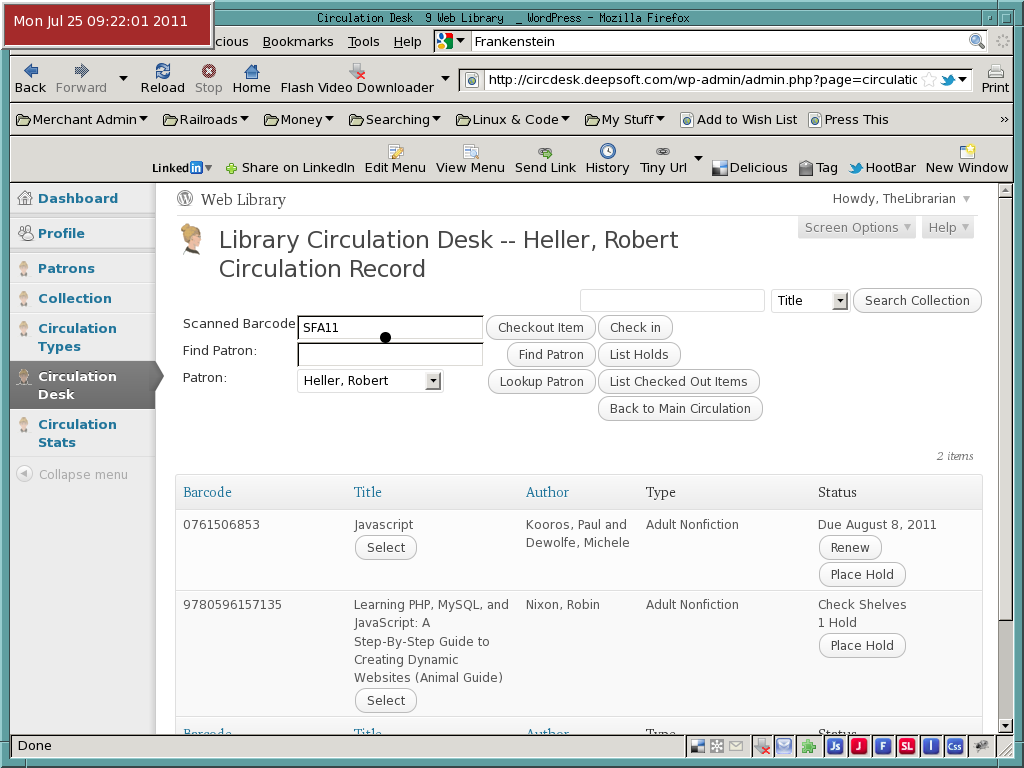
\includegraphics[width=4in]{PatronCirculationRecord} \caption{Circulation Record for a selected patron (Heller, Robert)}

\par\end{centering}

\centering{}\label{fig:PatronCirculationRecord} 
\end{figure}


This aspect of the \textit{Circulation Desk} page is shown when a
selected patron is looked up. It displays the selected patron's held
and checked out items. The \textbf{Lookup Barcode} button is changed
to a \textbf{Checkout Item} button. This button with cause the selected
item (barcode) to be checked out to the currently selected patron.
Again, an additional button is added to return to the main aspect
of the circulation desk page. A typical view of this page is shown
in Figure~\ref{fig:PatronCirculationRecord}.


\subsection{Circulation Hold List}

\label{sect:CirculationHoldList}

\begin{figure}[htbp]
\begin{centering}
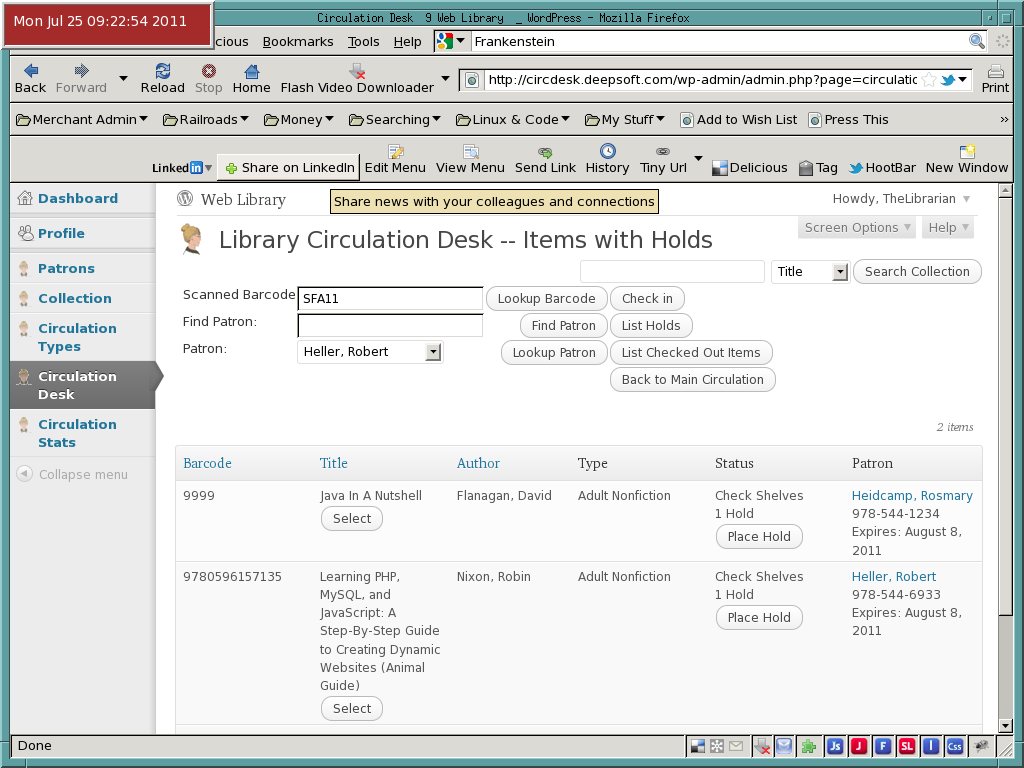
\includegraphics[width=4in]{CirculationHoldList} \caption{Circulation Hold List}

\par\end{centering}

\centering{}\label{fig:CirculationHoldList} 
\end{figure}


This aspect of the \textit{Circulation Desk} page lists all items
that currently have holds on them. An additional button is added to
return to the main aspect of the circulation desk page. A typical
view of this page is shown in Figure~\ref{fig:CirculationHoldList}.


\subsection{Circulation Checkout List}

\label{sect:CirculationCheckoutList}

\begin{figure}[htbp]
\begin{centering}
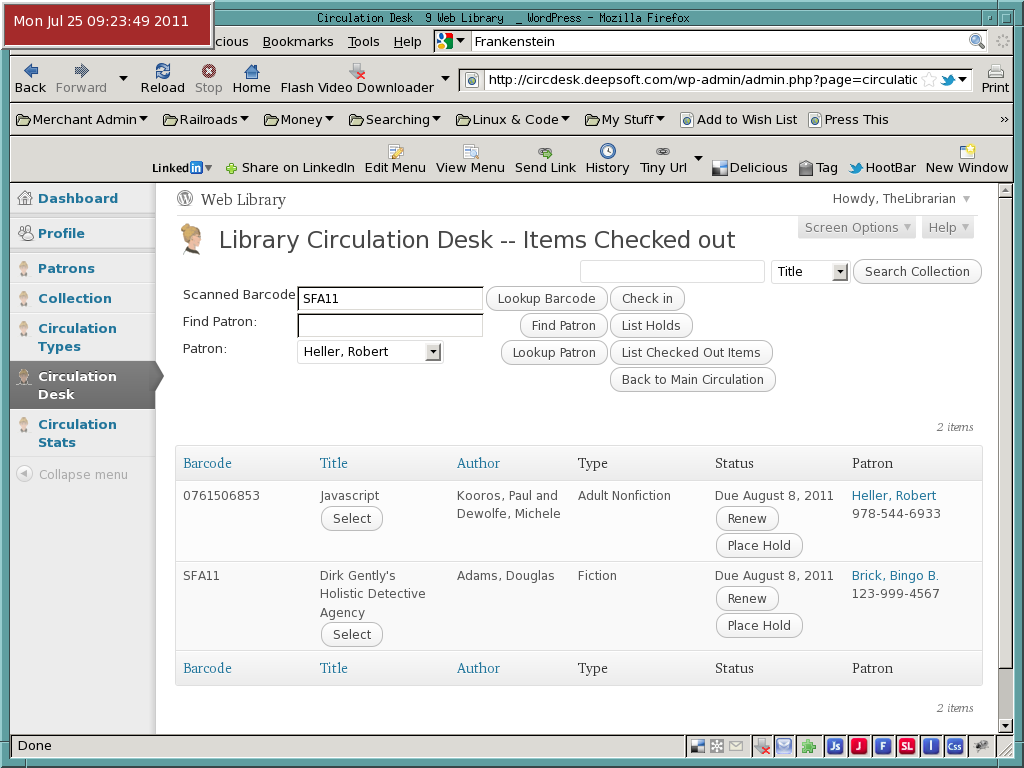
\includegraphics[width=4in]{CirculationCheckoutList} \caption{Circulation Checkout List}

\par\end{centering}

\centering{}\label{fig:CirculationCheckoutList} 
\end{figure}


This aspect of the \textit{Circulation Desk} page lists all items
that are currently checked out. An additional button is added to return
to the main aspect of the circulation desk page. A typical view of
this page is shown in Figure~\ref{fig:CirculationHoldList}.


\subsection{Circulation Checkin Page}

\label{sect:CirculationCheckinPage}

\begin{figure}[htbp]
\begin{centering}
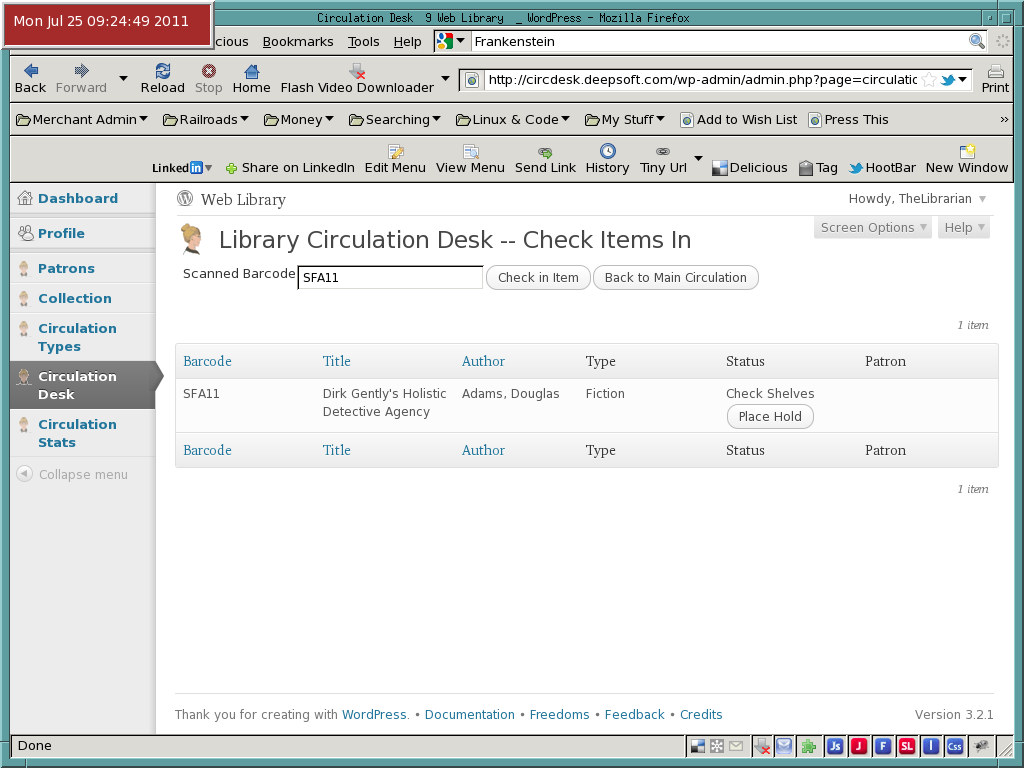
\includegraphics[width=4in]{CirculationCheckinPage} \caption{Circulation Checkin Page}

\par\end{centering}

\centering{}\label{fig:CirculationCheckinPage} 
\end{figure}


This aspect of the \textit{Circulation Desk} is used to check in returned
items. As items are checked in, they are listed as a verification
/ sanity check. A button is provided to return to the main aspect
of the circulation desk page. A typical view of this page is shown
in Figure~\ref{fig:CirculationCheckinPage}.


\section{Circulation Statistics}

\begin{figure}[htbp]
\begin{centering}
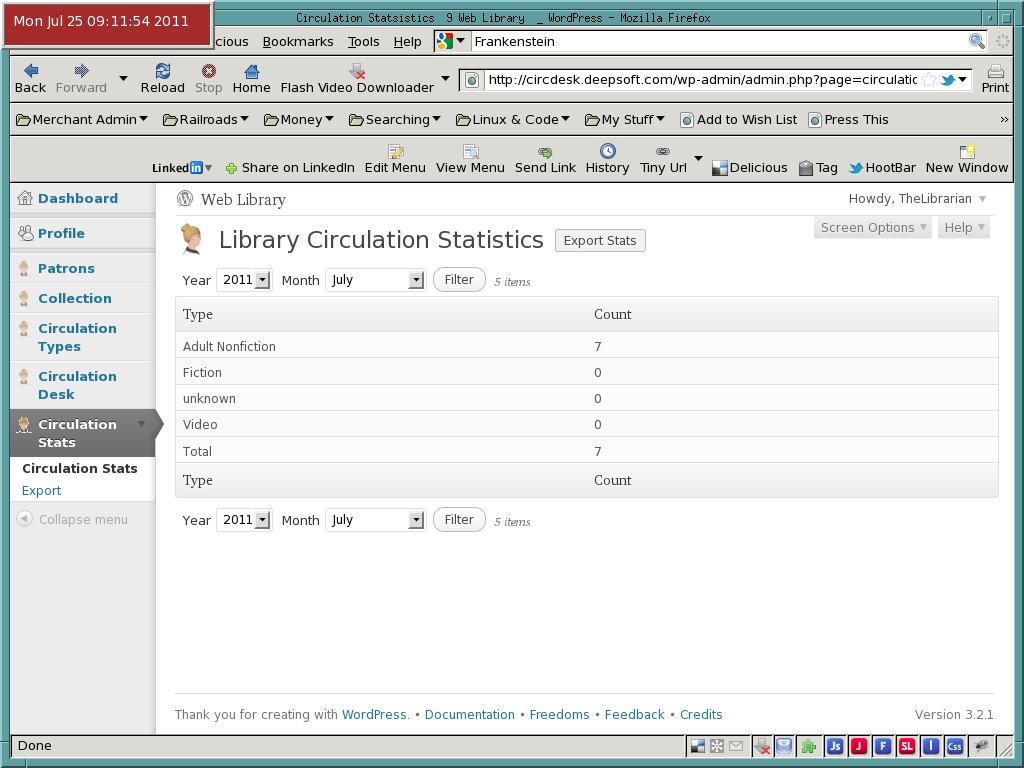
\includegraphics[width=4in]{CirculationTypesStatsList} \caption{Circulation Types Statistics List page}

\par\end{centering}

\centering{}\label{fig:CirculationTypesStatsList} 
\end{figure}


Finally, circulation statistics can be viewed and downloaded using
the circulation statistics pages. Circulation statistics can be listed
by month (shown in Figure~\ref{fig:CirculationTypesStatsList}) or
by monthly totals. The statistics can also be downloaded as CSV files.

\appendix
%dummy comment inserted by tex2lyx to ensure that this paragraph is not empty



\section{Stylesheet selectors used by the short codes (front end).}
\begin{description}
\item [{weblib-button}] This selector is used with both input and a tags
and defines how buttons look%
\footnote{With a (link) tags it makes the links look and act like buttons.%
}.


From \texttt{front.css}:


\begin{verbatim} /{*} All \textless{}input type=\char`\"{}submit\char`\"{}
...\textgreater{} and many \textless{}a href=\char`\"{}\char`\"{}...\textgreater{}
have class=\char`\"{}weblib-button\char`\"{} -- the links are meant
to look like buttons. I coded the submit buttons to have this class
as well as the \textless{}a href\textgreater{}'s, so that they would
all have the same styling. {*}/\par /{*} Common button styling {*}/
.weblib-button { border: outset 2px \#dcdad5; cursor: pointer; color:
\#000000; background-color: \#dcdad5; }\par .weblib-button:hover
{ font-weight: normal; color: \#000000; text-decoration: none; }\par /{*}
Links-as-buttons styling {*}/ a.weblib-button { height: 24px; white-space:
nowrap; /{*}padding: 2px;{*}/ padding: 0px; /{*} margin-top: 2px;
margin-bottom: 2px;{*}/ }\par a.weblib-button:link { font-weight:
normal; color: \#000000; text-decoration: none; }\par a.weblib-button:visited
{ color: \#000000; font-weight: normal; text-decoration: none; }
\end{verbatim}

\item [{weblib-total-results}] This selector is used with the total search
results count.


From \texttt{front.css}:


\begin{verbatim} .weblib-total-results { white-space: nowrap; font-weight:
bold; font-size: 150%;
 float: left; } \end{verbatim}

\item [{weblib-item-table}] This selector is used with the tags that contain
the search results.


From \texttt{front.css}:


\begin{verbatim} .weblib-item-content-block, .weblib-item-table {
display: table; } \end{verbatim}

\item [{weblib-item-row}] This selector is used with the tags that contain
a row of search results.


From \texttt{front.css}:


\begin{verbatim} .weblib-item-row { display: table-row; padding:
8px 0px; width: 100%;
} \end{verbatim}

\item [{weblib-item-index}] This selector is used with the tag that contains
the result index.


From \texttt{front.css}:


\begin{verbatim} .weblib-item-index { font-size: 150%;
 padding: 0px 4px; text-align: left; width: 5%;
} \end{verbatim}

\item [{weblib-item-element}] This is used with the tags for a single item
element.


From \texttt{front.css}:


\begin{verbatim} .weblib-item-element { display: table-cell; vertical-align:
top; padding: 2px; } \end{verbatim}

\item [{weblib-item-pagination-table}] This is used with the pagination
at the top and bottom of multipage results.


From \texttt{front.css}:


\begin{verbatim} .weblib-item-pagination-table { display: table;
width: 40%;
 margin: 2px 30%;
} \end{verbatim}

\item [{weblib-item-pagination}] This is used with the pagination at the
top and bottom of multipage results.


From \texttt{front.css}:


\begin{verbatim} .weblib-item-pagination { display: table-row; width:
100%;
 padding: 8px 0px; font-size: 120%;
}\par .weblib-item-pagination .pagelabel { vertical-align: top;
display: table-caption; padding: 2px; font-weight: bold; }\par .weblib-item-pagination
.pagelink { vertical-align: top; display: table-cell; margin: 0px;
}\par .weblib-item-pagination .pagenumform { white-space: nowrap;
width: 25%;
} \end{verbatim}

\item [{weblib-item-long}] This is used with long display of a single item.


From \texttt{front.css}:


\begin{verbatim} .weblib-item-long { display: table; } \end{verbatim}

\item [{weblib-item-head}] This is the item heading styling.
\item [{weblib-item-left}] This is the left side of the long item display.


From \texttt{front.css}:


\begin{verbatim} .weblib-item-left { width: 90%;
} \end{verbatim}

\item [{weblib-item-content-block}] This is the long item content block.


From \texttt{front.css}:


\begin{verbatim} .weblib-item-content-block, .weblib-item-table {
display: table; } \end{verbatim}

\item [{weblib-item-content-element}] This is the long item content element.


From \texttt{front.css}:


\begin{verbatim} .weblib-item-content-element { display: table-row;
} \end{verbatim}

\item [{weblib-item-left-head}] This is the long item left heading.


From \texttt{front.css}:


\begin{verbatim} .weblib-item-left-head { font-weight: bold; text-align:
right; display: table-cell; padding: 2px; } \end{verbatim}

\item [{weblib-item-left-content}] This is the long item left content.


From \texttt{front.css}:


\begin{verbatim} .weblib-item-left-content { text-align: left; display:
table-cell; padding: 2px; } \end{verbatim}

\item [{weblib-item-author}] This is the styling of the author name.


From \texttt{front.css}:


\begin{verbatim} .weblib-item-author { text-decoration: underline;
} \end{verbatim}

\item [{weblib-item-title}] This is the styling of the title.


From \texttt{front.css}:


\begin{verbatim} .weblib-item-title { font-weight: bold; } \end{verbatim}

\item [{weblib-item-right}] This is the styling of the right side of the
long item display.


From \texttt{front.css}:


\begin{verbatim} .weblib-item-right { } \end{verbatim}

\item [{weblib-item-center-head}] This is the styling of the keyword heading
of the heading.


From \texttt{front.css}:


\begin{verbatim} .weblib-item-center-head { font-weight: bold; text-align:
center; display: table-cell; padding: 2px; } \end{verbatim}

\item [{weblib-item-keyword-list}] This is the styling of the keyword list.


From \texttt{front.css}:


\begin{verbatim} .weblib-item-keyword-list { text-align: center;
display: table-cell; padding: 2px; } \end{verbatim}

\item [{weblib-item-thumb}] This is the styling of the thumbnail image.


From \texttt{front.css}:


\begin{verbatim} .weblib-item-thumb { padding: 0px 4px; }\par .weblib-item-thumb
img { min-width: 48px; min-height: 72px; } \end{verbatim}

\item [{weblib-item-holdbutton}] This is the styling of the hold (request)
button.


From \texttt{front.css}:


\begin{verbatim} .weblib-item-holdbutton { } \end{verbatim}

\item [{weblib-item-brief}] This is used to style the brief item display.


From \texttt{front.css}:


\begin{verbatim} .weblib-item-brief { } \end{verbatim}

\item [{weblib-item-info}] This is used to style the item info.


From \texttt{front.css}:


\begin{verbatim} .weblib-item-info { width: 85%;
} \end{verbatim} \end{description}

\end{document}
